\documentclass[final]{beamer}

% ====================
% Packages
% ====================

\usepackage[T1]{fontenc}
 \usepackage[utf8]{luainputenc}
\usepackage{lmodern}
\usepackage[size=custom, width=120,height=72, scale=1.1]{beamerposter}
\usetheme{gemini}
\usecolortheme{cam}
\usepackage{graphicx}
\usepackage{booktabs}
\usepackage{tikz}
\usepackage{pgfplots}
\pgfplotsset{compat=1.14}
\usepackage{anyfontsize}
\usepackage{fontawesome5}
\usepackage{algorithm}
\usepackage{algpseudocode}
\usepackage[backend=biber,style=ieee]{biblatex}

\addbibresource{references.bib}

\graphicspath{{../figures/}}

% ====================
% Lengths
% ====================

% If you have N columns, choose \sepwidth and \colwidth such that
% (N+1)*\sepwidth + N*\colwidth = \paperwidth
\newlength{\sepwidth}
\newlength{\colwidth}
\setlength{\sepwidth}{0.025\paperwidth}
\setlength{\colwidth}{0.3\paperwidth}

\newcommand{\separatorcolumn}{\begin{column}{\sepwidth}\end{column}}
\newcommand\mycalc[1]{\directlua{tex.sprint(#1)}}



% ====================
% Title
% ====================

\title{Practical Analysis of Hybrid Sorting Algorithms}

\author{Joshua Arulsamy}

\institute[shortinst]{Department of Electrical Engineering and Computer Science, University of Wyoming}

% ====================
% Footer (optional)
% ====================

\footercontent{
  \faGithub\ \href{https://github.com/uwyo-mallet/Hybrid-Sorting-Optimization}{https://github.com/uwyo-mallet/Hybrid-Sorting-Optimization} \hfill
  Undergraduate Research and Inquiry Day 2023 \hfill \hfill
  \href{mailto:jarulsam@uwyo.edu}{jarulsam@uwyo.edu}
}
% (can be left out to remove footer)

% ====================
% Logo (optional)
% ====================

% use this to include logos on the left and/or right side of the header:
% Left: institution
 \logoleft{
\includegraphics[height=2.9cm]{logos/New_UWSignature_1_line_White_Web.png}}
% Right: funding agencies and other affilations
% \logoright{
\includegraphics[height=2.5cm]{logos/WRSP/abbreviated/UWabbreviated_V_WRSP_white.png}}
% ====================
% Body
% ====================

\begin{document}

% \addtobeamertemplate{block begin}{\vskip -\bigskipamount}{}
% \addtobeamertemplate{block end}{}{\vskip -\bigskipamount}

\begin{frame}[t]
	\begin{columns}[t]
		\separatorcolumn

		\begin{column}{\colwidth}

			\begin{block}{Introduction}
				\begin{itemize}
					\item Most applications require data to be arranged in a certain order.
					      The procedure of reordering data according to some comparator is
					      called sorting. Sorting can be found in nearly every computer
					      system today.
					\item The near omnipresent need for
					      performant sorting implementations has resulted in most major
					      programming languages including a type-generic sorting function
					      within their standard libraries.
					\item This research analyzes a wide variety of sorting
					      algorithm implementations across varying system architectures to
					      determine optimal parameter configurations for hybrid sorting
					      algorithms.
					\item This research also proposes a new performant standard
					      sorting implementation for GNU's C standard library leveraging
					      Mergesort, insertion sort, and sorting networks.
				\end{itemize}
			\end{block}

			\begin{block}{Background}
				\begin{itemize}
					\item Substantial effort has been spent on the analysis of
					      sorting algorithms. Typically, two major characteristics
					      are considered when studying sorting algorithms; space
					      and time complexity.
					\item Existing analysis of popular sorting algorithms, such as Quicksort
					      and Mergesort, place substantial emphasis on their excellent
					      asymptotic complexity in the average case\parencite{glibc}.
					\item Asymptotic complexity alone does not describe the
					      practical performance of these algorithms. While Mergesort may
					      have a better asymptotic time complexity in the worst case than
					      insertion sort, for small inputs, insertion sort typically
					      outperforms Mergesort by avoiding the overhead of recursive calls.
				\end{itemize}
			\end{block}

			\begin{block}{Proposed Algorithms}
				\begin{itemize}
					\item The proposed algorithm is a highly-optimized version of
					      Mergesort leveraging both insertion sort and a network
					      sorting algorithm.
					\item During recursive calls of conventional Mergesort, if the
					      subarray's length is less than a threshold value,
					      insertion sort is used instead.
					\item In instances where a subarray contains less than 5
					      elements, a comparison-optimal network sorting algorithm
					      is used instead.
					\item In practice, this offers significant performance gains,
					      as the maximum recursion depth of Mergesort is limited.
				\end{itemize}
			\end{block}
		\end{column}

		\separatorcolumn

		\begin{column}{\colwidth}

			\begin{block}{Experimental Setup}

				A small subset of algorithms were chosen for evaluation.
				Primarily, algorithms utilized within standard library
				implementations are of particular interest, since they are
				typically highly performant in the general case. Other
				complementary algorithms which perform exceptionally well in
				specific scenarios were also evaluated. Since this analysis is
				focused on analyzing and improving existing implementations,
				general purpose sorting function were taken from various standard
				libraries, such as GNU's libc\parencite{glibc} and musl
				libc\parencite{musl_libc}.

				\begin{enumerate}
					\item \textbf{Each algorithm is timed while sorting the same data using a variety of threshold values.} This is repeated 1,000 times. The mean is calculated for each
					      algorithm. This is done to minimize noise (time
					      inaccuracy, other processes on the test system, etc.)
					      during data collection.
					\item \textbf{Each algorithm configuration is tested on a
						      variety of platforms}. To determine whether the
					      algorithms perform well across a variety of
					      architectures, each test is repeated on different,
					      commonly used systems.
					\item \textbf{Results are analyzed}. The performance
					      difference from the standard built-in sorting function
					      \texttt{qsort} is calculated and plotted. This function
					      serves as a baseline to compare performance against. The
					      variance of improvement from system to system is also
					      plotted.
				\end{enumerate}
			\end{block}

			\begin{block}{Results}

				Et rutrum ex euismod vel. Pellentesque ultricies, velit in fermentum
				vestibulum, lectus nisi pretium nibh, sit amet aliquam lectus augue vel
				velit. Suspendisse rhoncus massa porttitor augue feugiat molestie. Sed
				molestie ut orci nec malesuada. Sed ultricies feugiat est fringilla
				posuere.

				\begin{figure}[h]
					\centering
					\makebox[0.75\columnwidth]{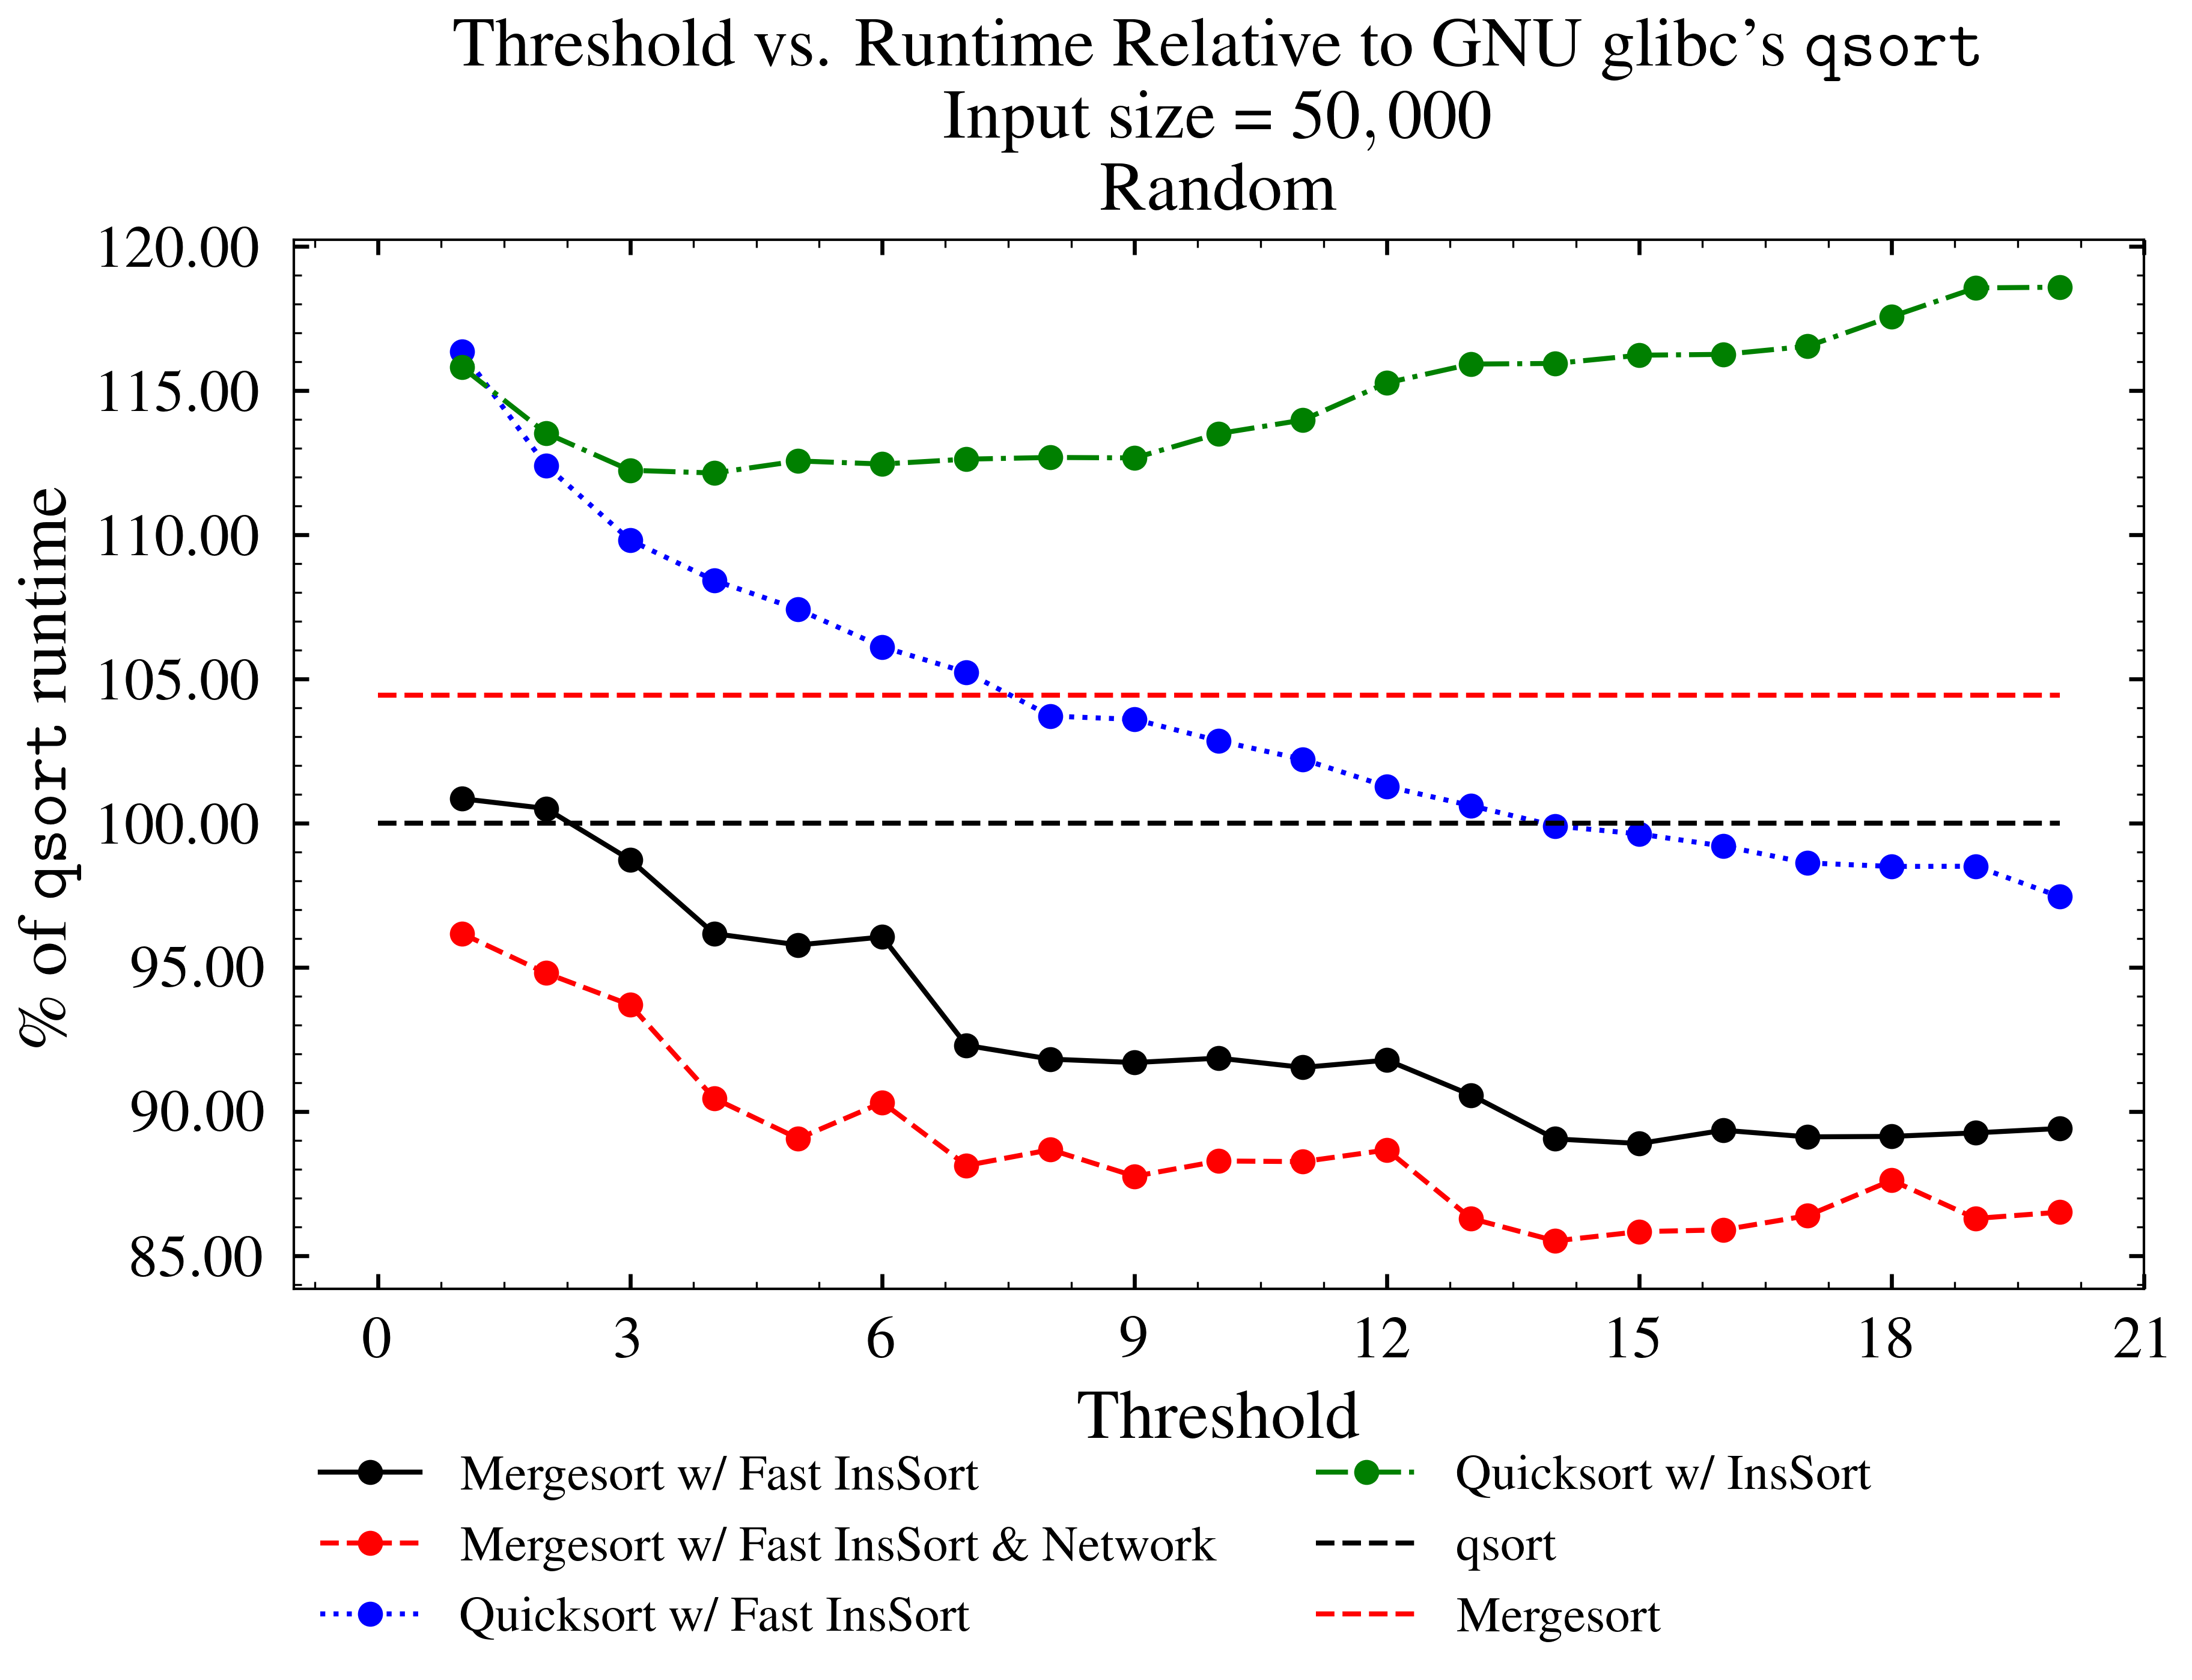
\includegraphics[width=0.75\columnwidth]{random}}
					\caption{Random}
					\label{fig:random}
				\end{figure}
				% \begin{figure}[h]
				% 	\centering
				% 	\makebox[0.75\columnwidth]{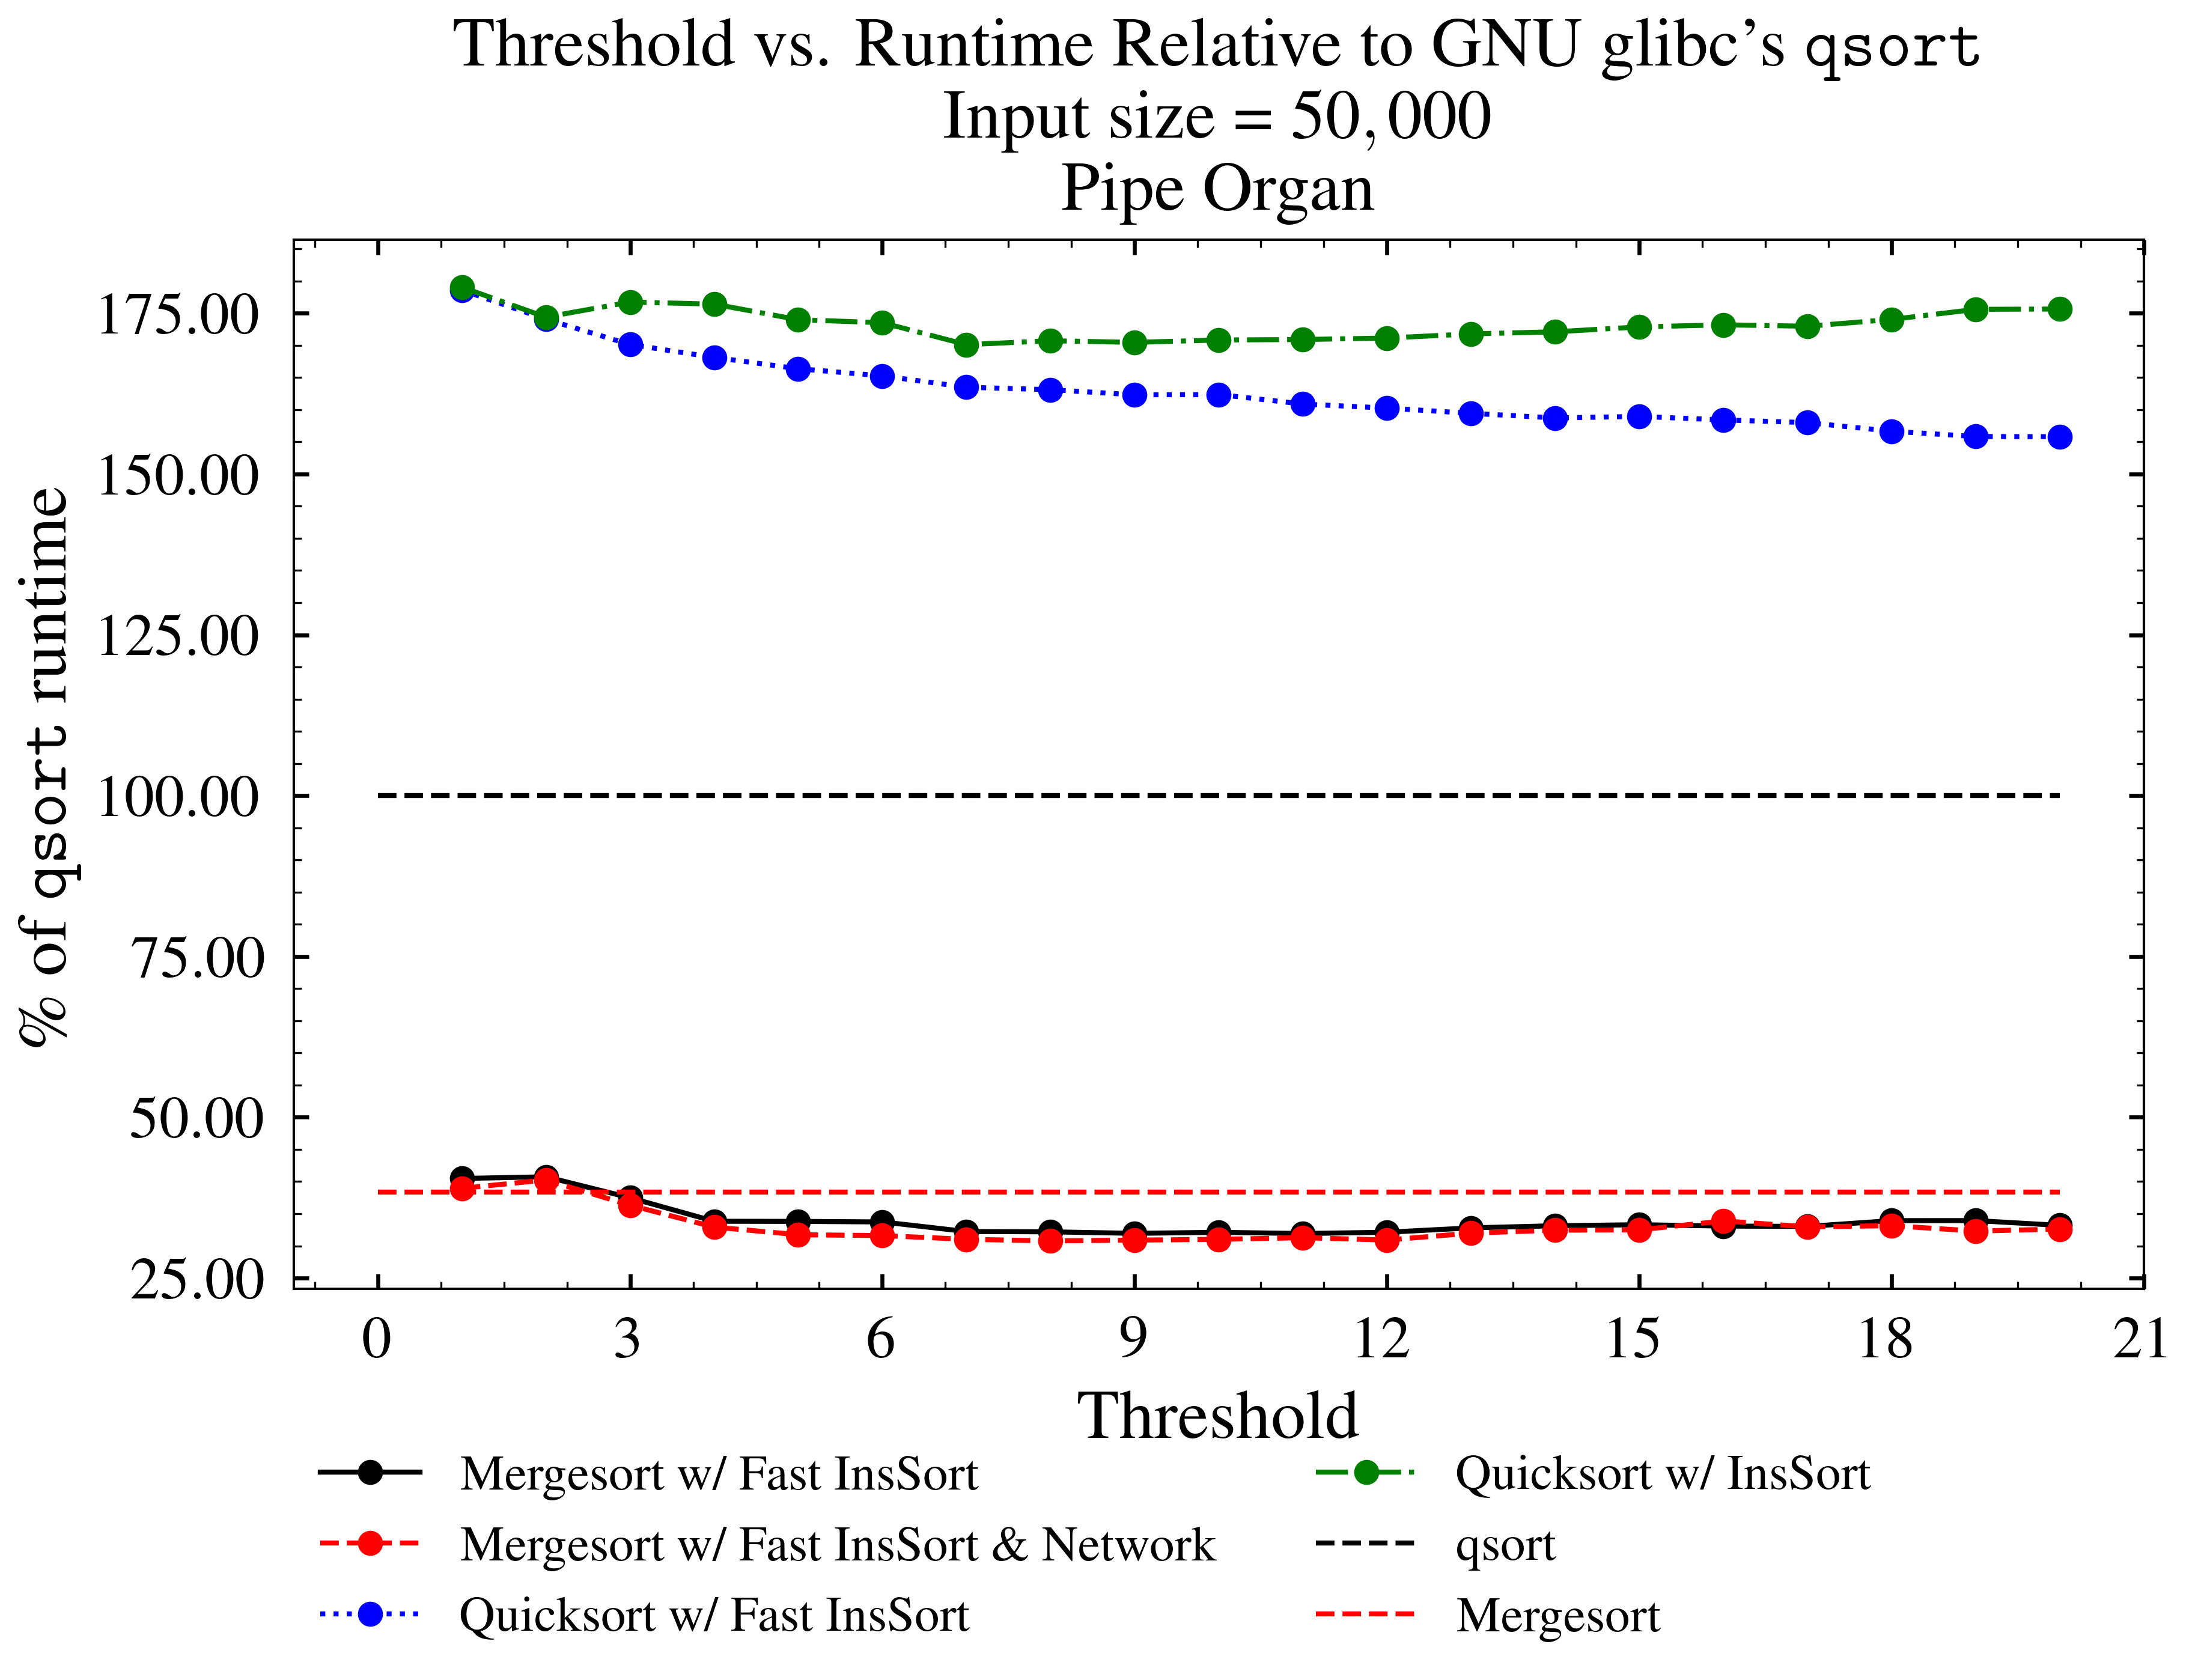
\includegraphics[width=0.75\columnwidth]{pipe_organ}}
				% 	\caption{Pipe Organ}
				% 	\label{fig:pipe_organ}
				% \end{figure}
				% \begin{figure}[h]
				% 	\centering
				% 	\makebox[0.75\columnwidth]{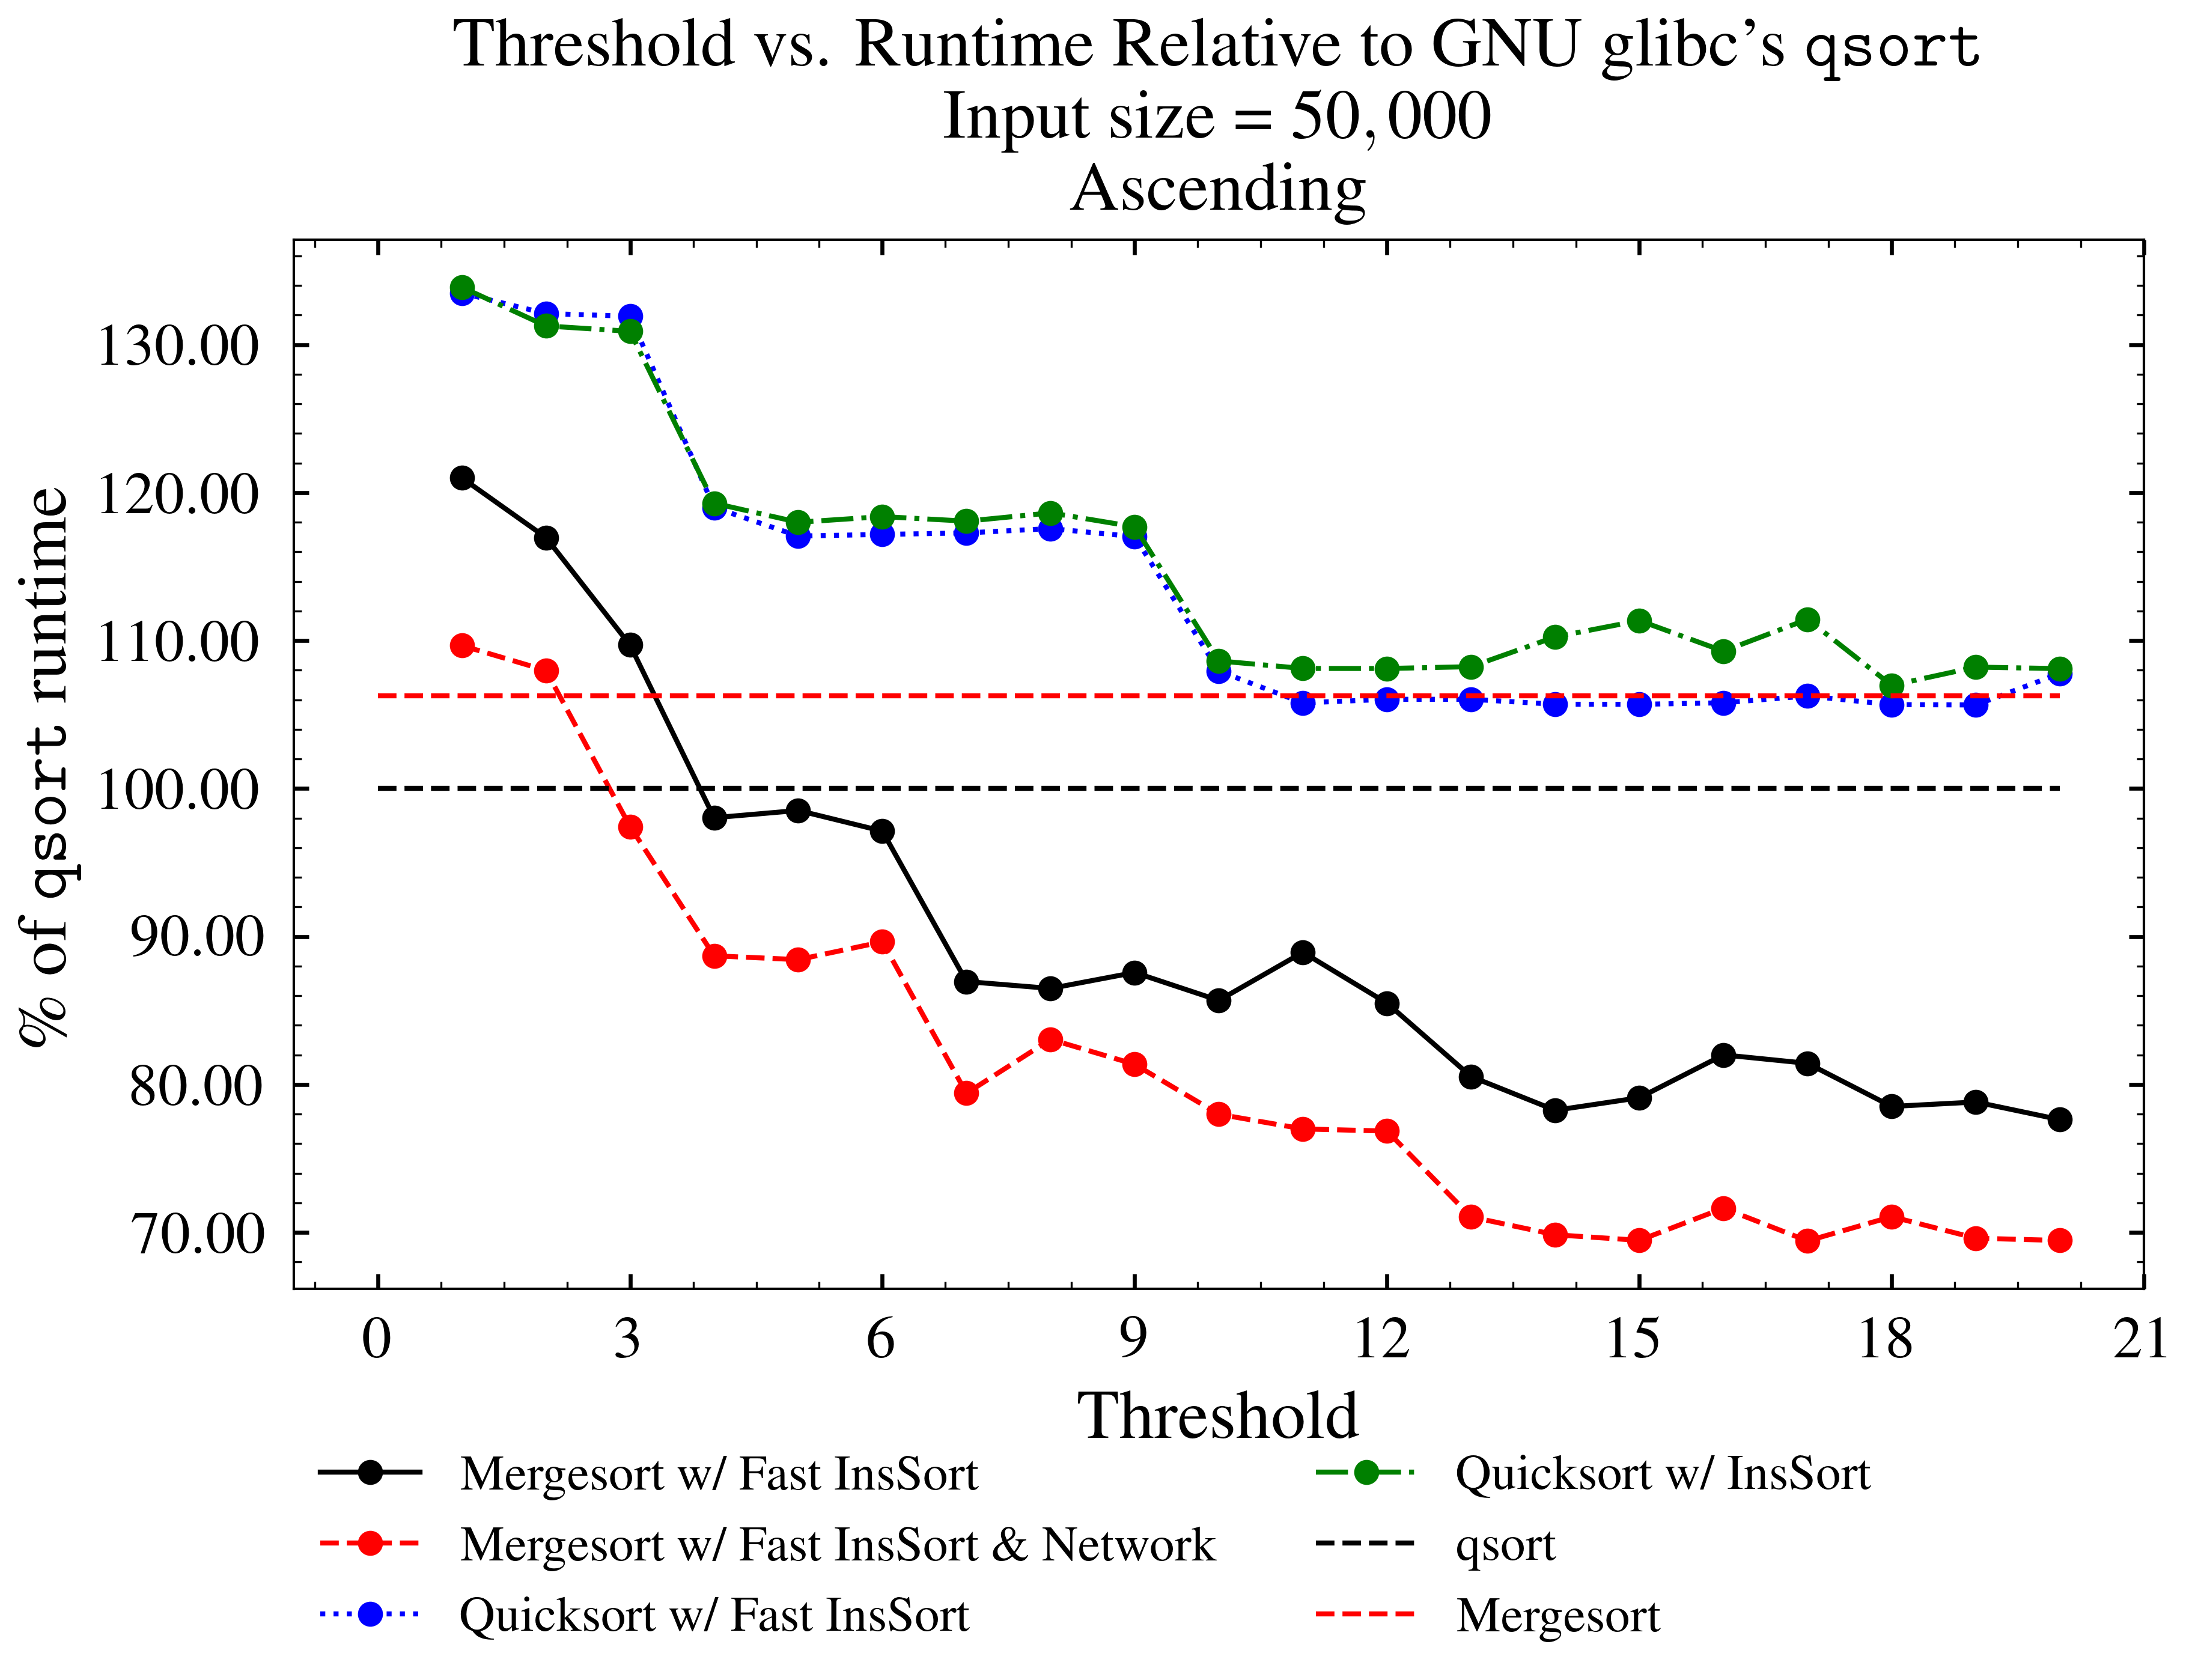
\includegraphics[width=0.75\columnwidth]{ascending}}
				% 	\caption{Ascending}
				% 	\label{fig:ascending}
				% \end{figure}
				% \begin{figure}[h]
				% 	\centering
				% 	\makebox[0.75\columnwidth]{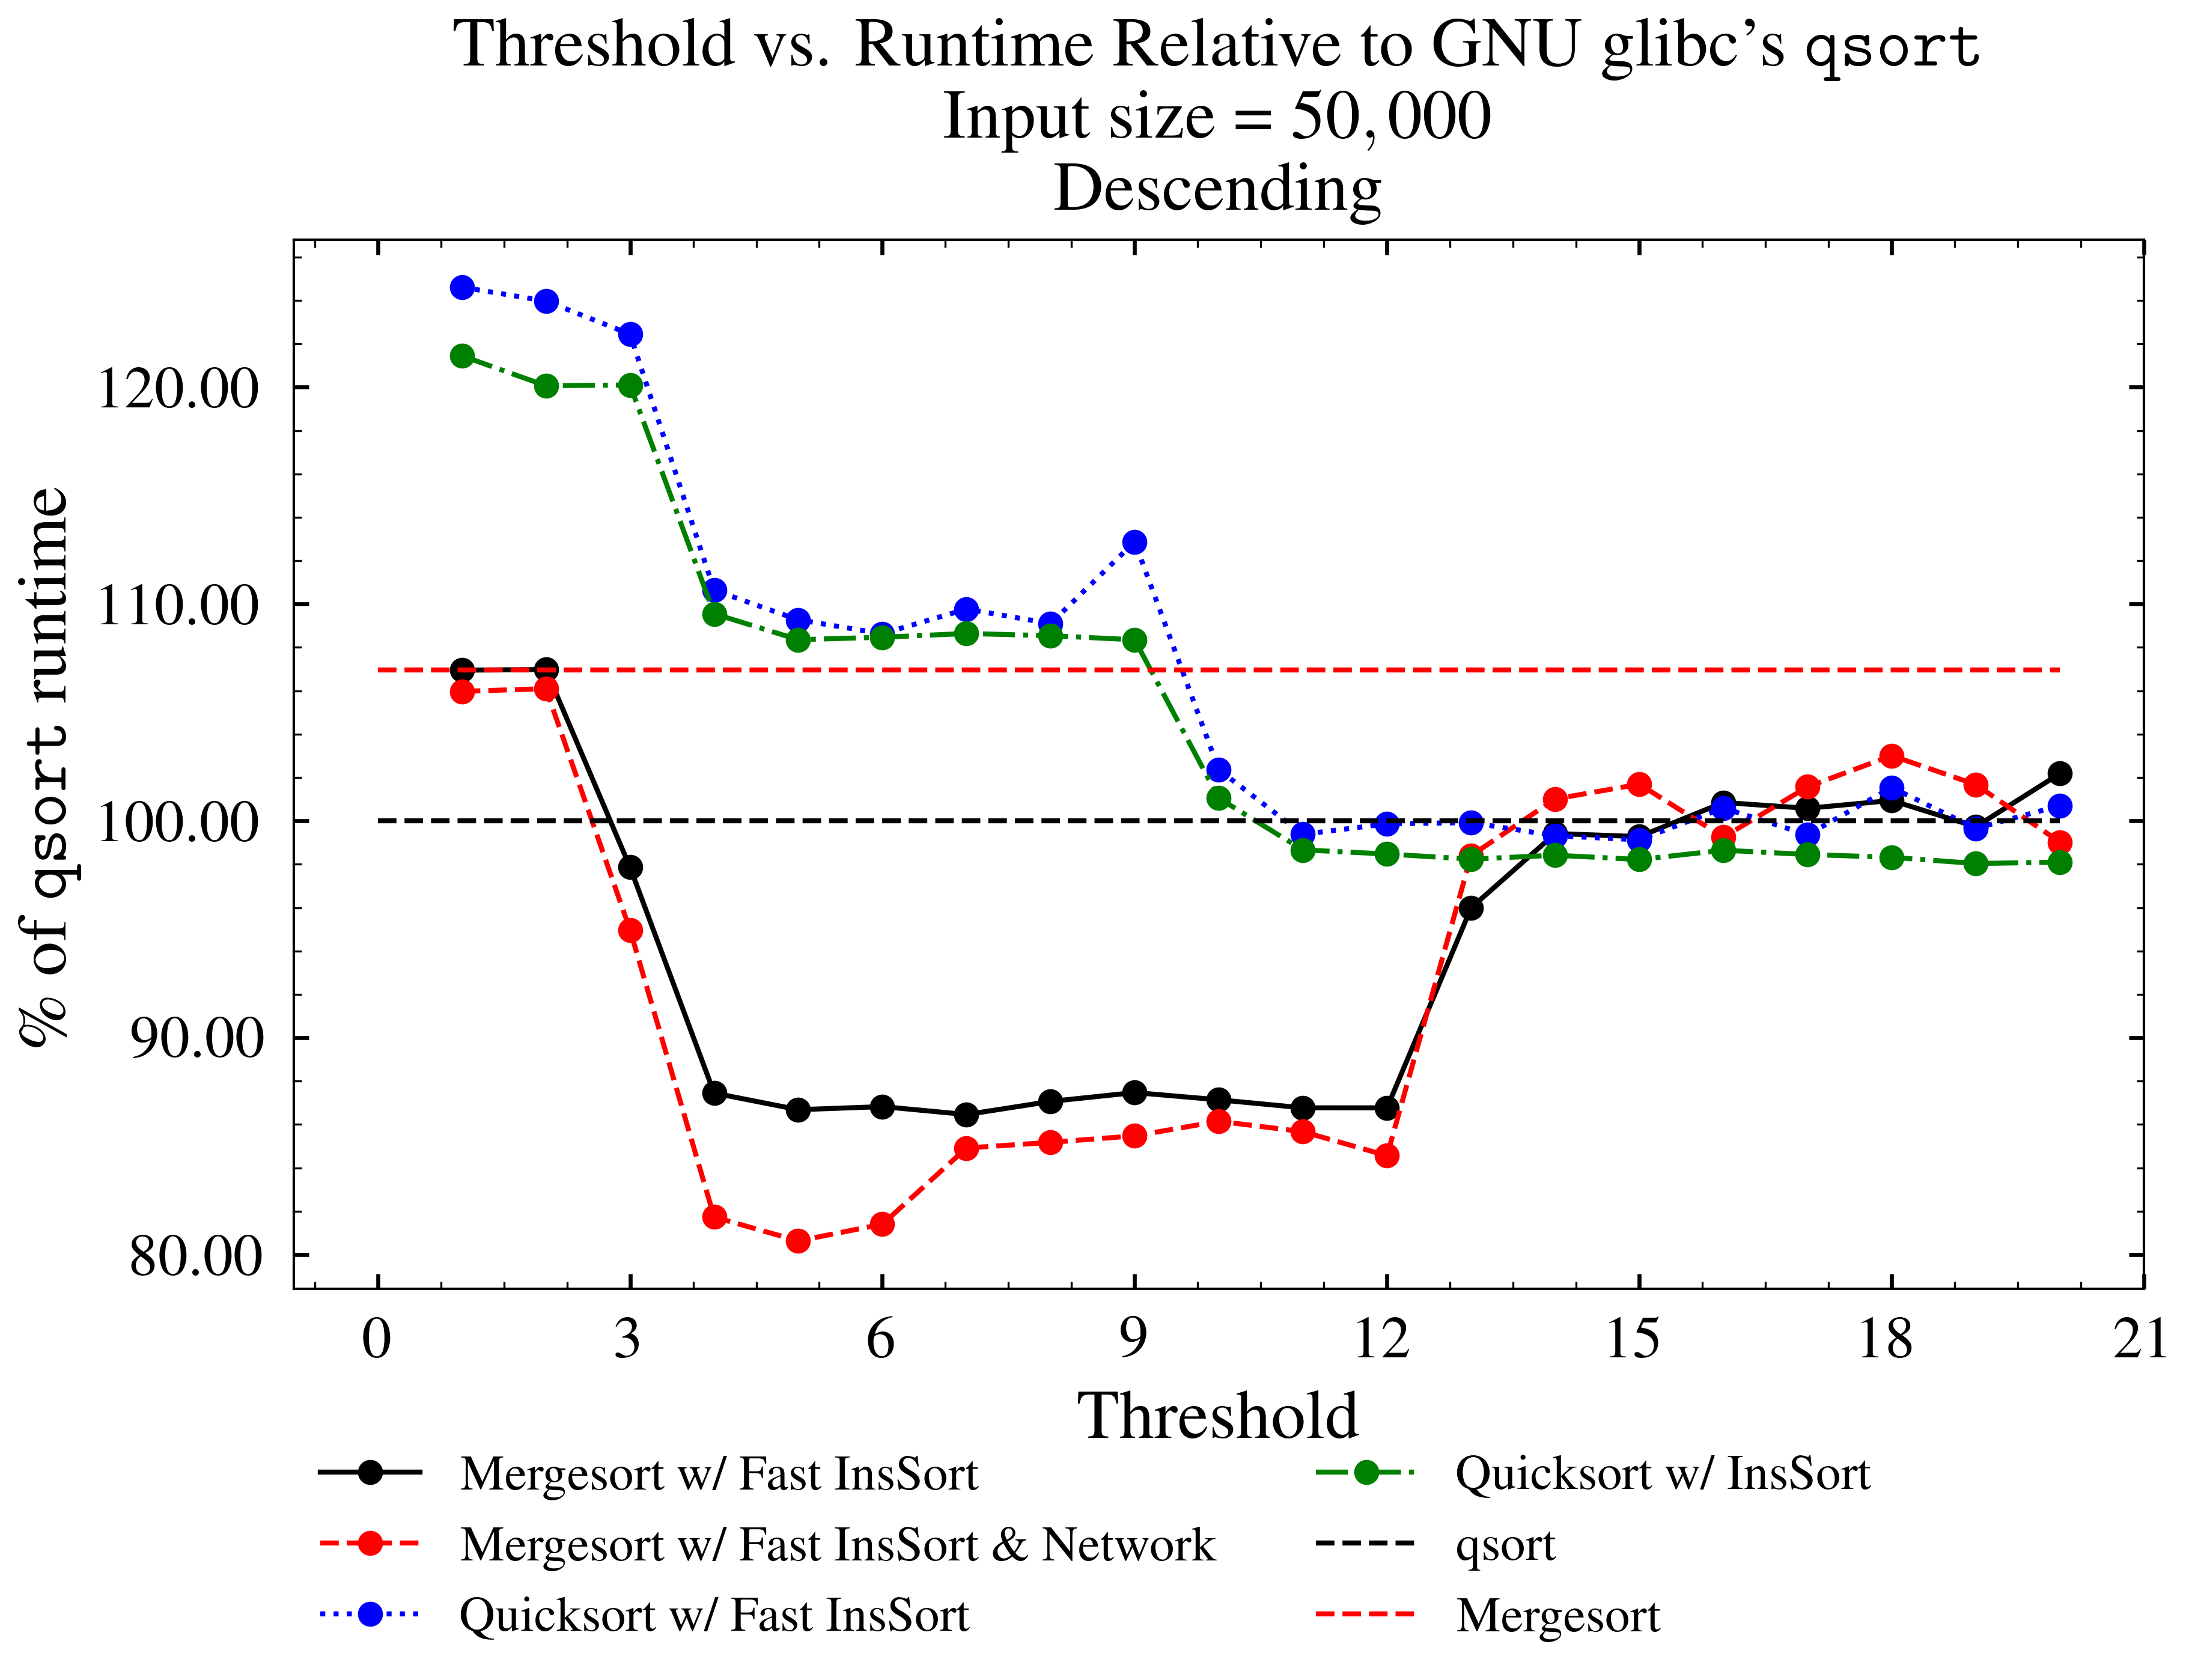
\includegraphics[width=0.75\columnwidth]{descending}}
				% 	\caption{Descending}
				% 	\label{fig:descending}
				% \end{figure}
				% \begin{figure}[h]
				% 	\centering
				% 	\makebox[0.75\columnwidth]{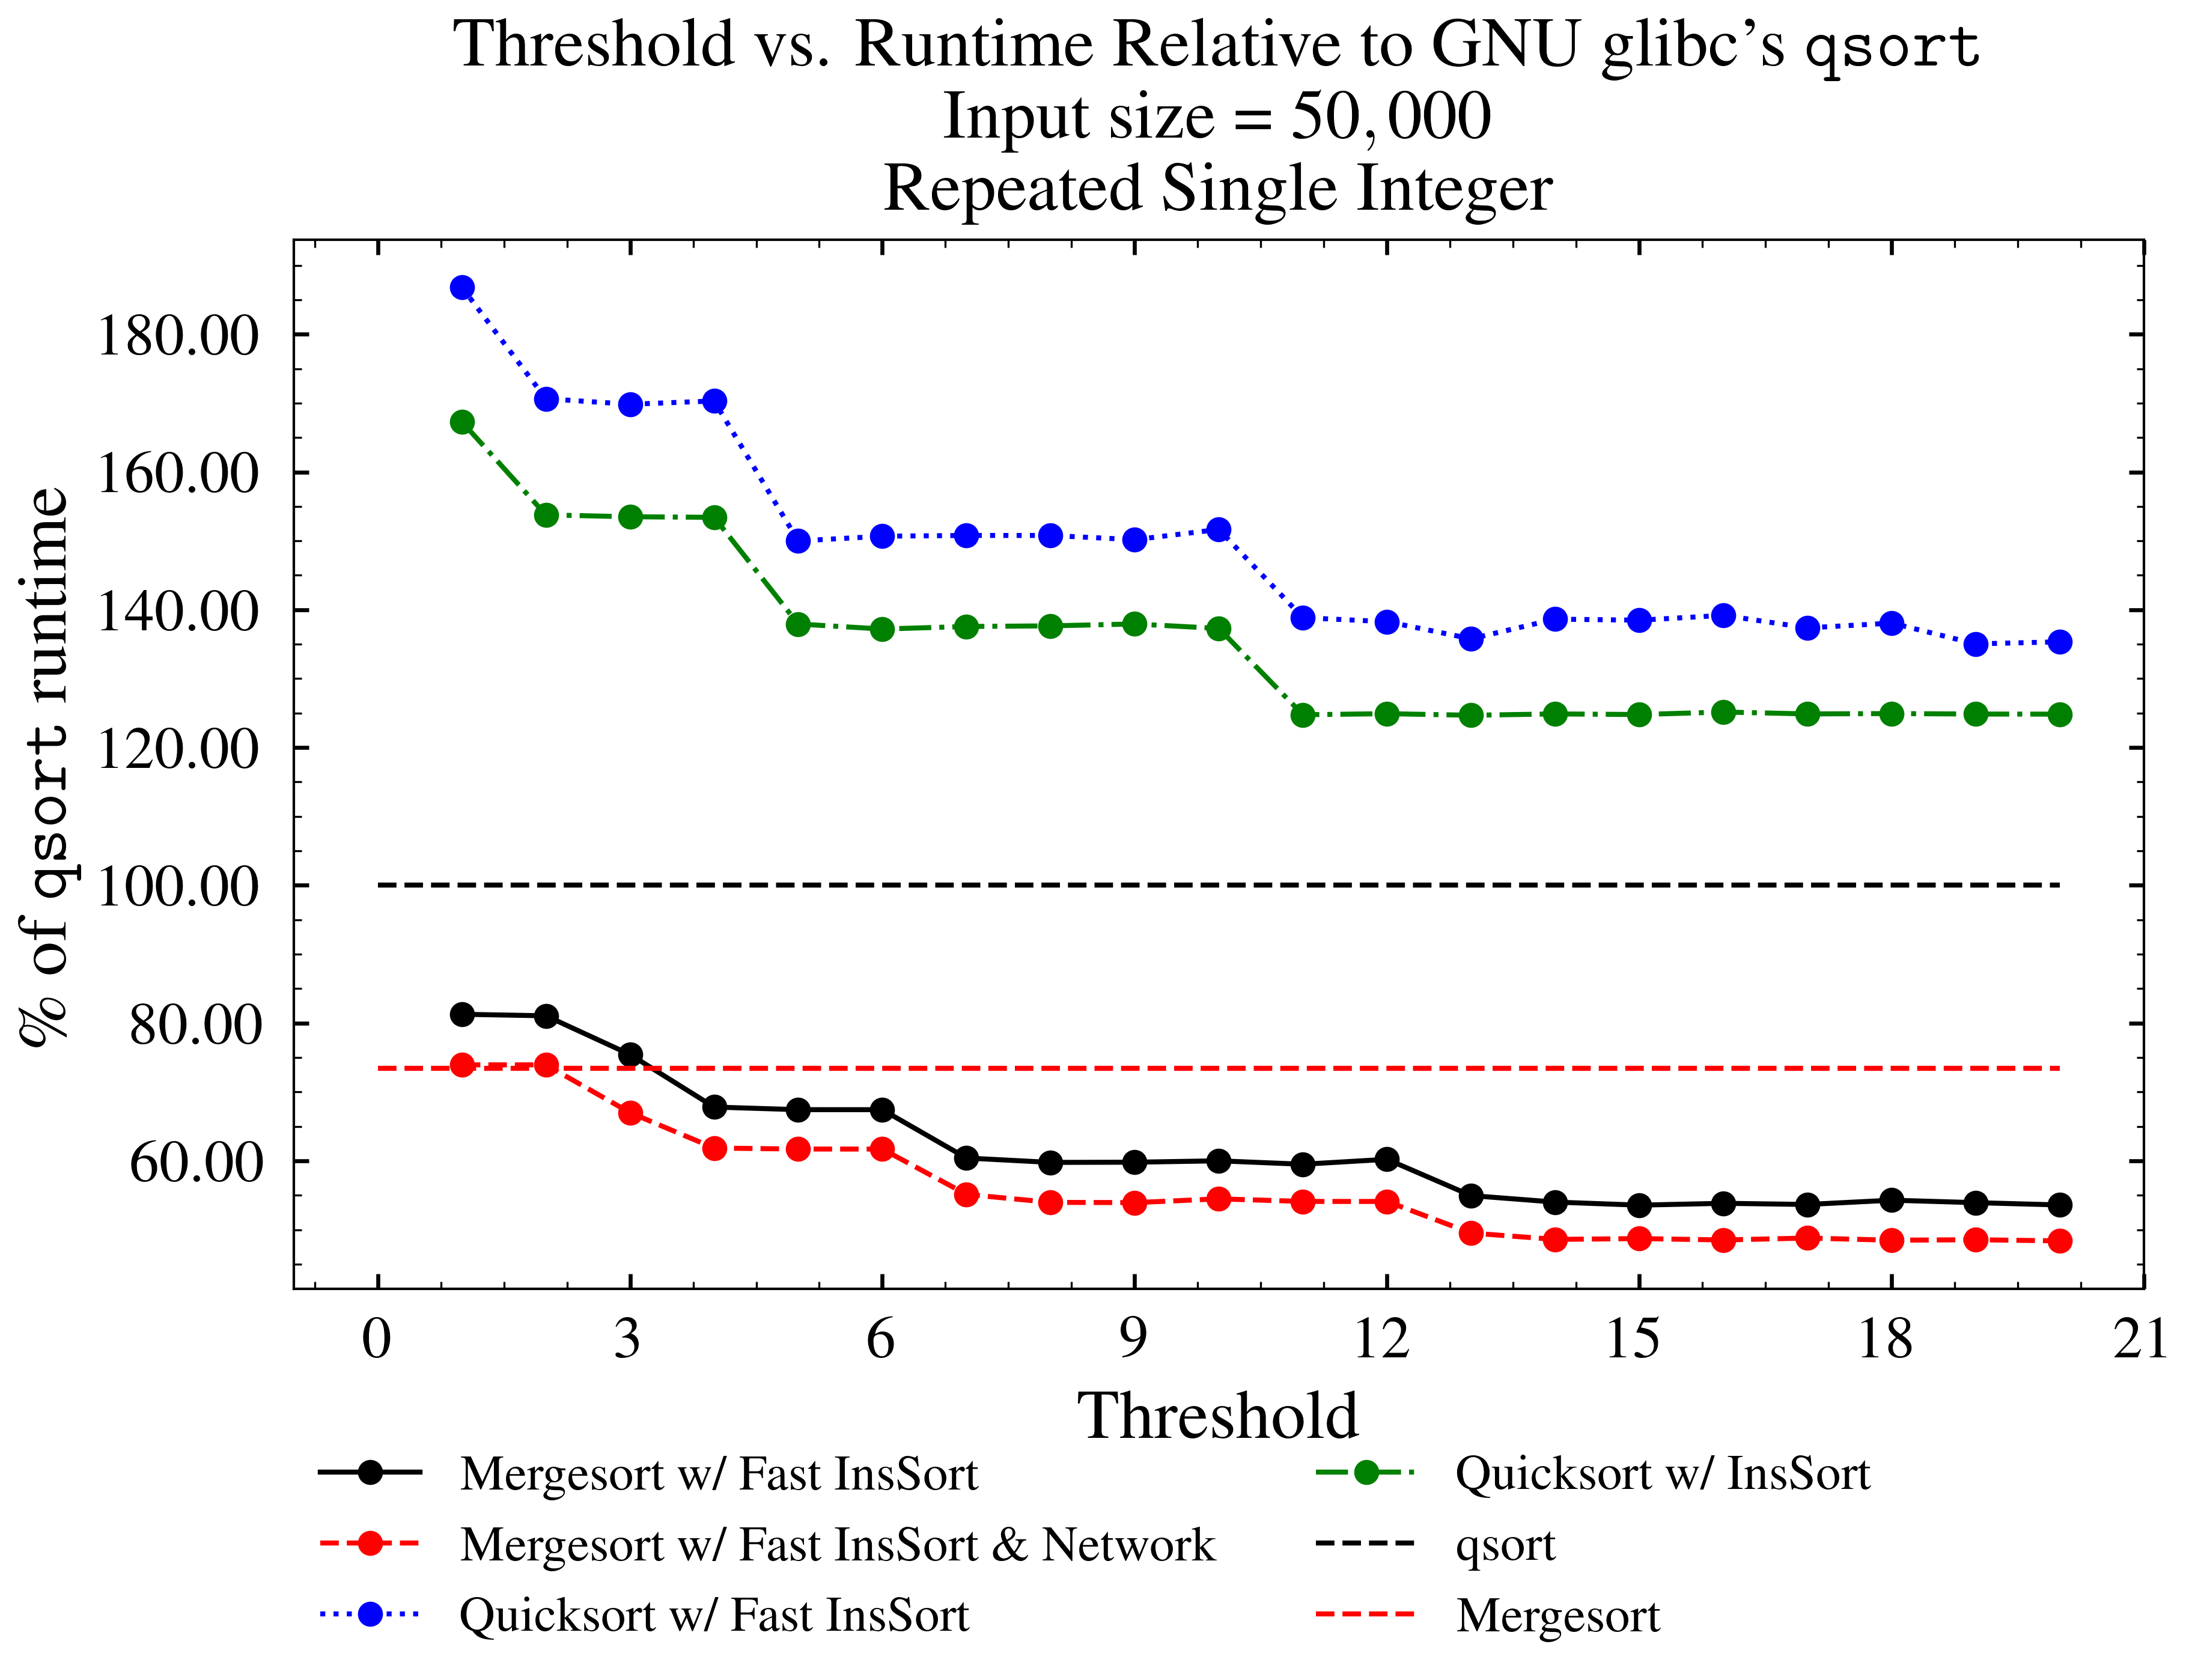
\includegraphics[width=0.75\columnwidth]{single_num}}
				% 	\caption{Single Num}
				% 	\label{fig:single_num}
				% \end{figure}

			\end{block}

			% \begin{block}{Nam cursus consequat egestas}

			% 	Nulla eget sem quam. Ut aliquam volutpat nisi vestibulum convallis. Nunc a
			% 	lectus et eros facilisis hendrerit eu non urna. Interdum et malesuada fames
			% 	ac ante \textit{ipsum primis} in faucibus. Etiam sit amet velit eget sem
			% 	euismod tristique. Praesent enim erat, porta vel mattis sed, pharetra sed
			% 	ipsum. Morbi commodo condimentum massa, \textit{tempus venenatis} massa
			% 	hendrerit quis. Maecenas sed porta est. Praesent mollis interdum lectus,
			% 	sit amet sollicitudin risus tincidunt non.

			% 	Etiam sit amet tempus lorem, aliquet condimentum velit. Donec et nibh
			% 	consequat, sagittis ex eget, dictum orci. Etiam quis semper ante. Ut eu
			% 	mauris purus. Proin nec consectetur ligula. Mauris pretium molestie
			% 	ullamcorper. Integer nisi neque, aliquet et odio non, sagittis porta justo.

			% 	\begin{itemize}
			% 		\item \textbf{Sed consequat} id ante vel efficitur. Praesent congue massa
			% 		      sed est scelerisque, elementum mollis augue iaculis.
			% 		      \begin{itemize}
			% 			      \item In sed est finibus, vulputate
			% 			            nunc gravida, pulvinar lorem. In maximus nunc dolor, sed auctor eros
			% 			            porttitor quis.
			% 			      \item Fusce ornare dignissim nisi. Nam sit amet risus vel lacus
			% 			            tempor tincidunt eu a arcu.
			% 			      \item Donec rhoncus vestibulum erat, quis aliquam leo
			% 			            gravida egestas.
			% 		      \end{itemize}
			% 		\item \textbf{Sed luctus, elit sit amet} dictum maximus, diam dolor
			% 		      faucibus purus, sed lobortis justo erat id turpis.
			% 		\item \textbf{Pellentesque facilisis dolor in leo} bibendum congue.
			% 		      Maecenas congue finibus justo, vitae eleifend urna facilisis at.
			% 	\end{itemize}

			% \end{block}

		\end{column}

		\separatorcolumn

		\begin{column}{\colwidth}

			\begin{exampleblock}{A highlighted block containing some math}

				A different kind of highlighted block.

				$$
					\int_{-\infty}^{\infty} e^{-x^2}\,dx = \sqrt{\pi}
				$$

				Interdum et malesuada fames $\{1, 4, 9, \ldots\}$ ac ante ipsum primis in
				faucibus. Cras eleifend dolor eu nulla suscipit suscipit. Sed lobortis non
				felis id vulputate.

				\heading{A heading inside a block}

				Praesent consectetur mi $x^2 + y^2$ metus, nec vestibulum justo viverra
				nec. Proin eget nulla pretium, egestas magna aliquam, mollis neque. Vivamus
				dictum $\mathbf{u}^\intercal\mathbf{v}$ sagittis odio, vel porta erat
				congue sed. Maecenas ut dolor quis arcu auctor porttitor.

				\heading{Another heading inside a block}

				Sed augue erat, scelerisque a purus ultricies, placerat porttitor neque.
				Donec $P(y \mid x)$ fermentum consectetur $\nabla_x P(y \mid x)$ sapien
				sagittis egestas. Duis eget leo euismod nunc viverra imperdiet nec id
				justo.

			\end{exampleblock}

			\begin{block}{Nullam vel erat at velit convallis laoreet}

				Class aptent taciti sociosqu ad litora torquent per conubia nostra, per
				inceptos himenaeos. Phasellus libero enim, gravida sed erat sit amet,
				scelerisque congue diam. Fusce dapibus dui ut augue pulvinar iaculis.

				\begin{table}
					\centering
					\begin{tabular}{l r r c}
						\toprule
						\textbf{First column} & \textbf{Second column} & \textbf{Third column} & \textbf{Fourth} \\
						\midrule
						Foo                   & 13.37                  & 384,394               & $\alpha$        \\
						Bar                   & 2.17                   & 1,392                 & $\beta$         \\
						Baz                   & 3.14                   & 83,742                & $\delta$        \\
						Qux                   & 7.59                   & 974                   & $\gamma$        \\
						\bottomrule
					\end{tabular}
					\caption{A table caption.}
				\end{table}

				Donec quis posuere ligula. Nunc feugiat elit a mi malesuada consequat. Sed
				imperdiet augue ac nibh aliquet tristique. Aenean eu tortor vulputate,
				eleifend lorem in, dictum urna. Proin auctor ante in augue tincidunt
				tempor. Proin pellentesque vulputate odio, ac gravida nulla posuere
				efficitur. Aenean at velit vel dolor blandit molestie. Mauris laoreet
				commodo quam, non luctus nibh ullamcorper in. Class aptent taciti sociosqu
				ad litora torquent per conubia nostra, per inceptos himenaeos.
			\end{block}

			\begin{block}{References}
				\footnotesize{\printbibliography}
			\end{block}
		\end{column}

		\separatorcolumn
	\end{columns}
\end{frame}

\end{document}
